\section{Circuit-awareness and PhEDEx}

PhEDEx consists of a set of software agents interacting with a central database. Circuit-awareness can be integrated into PhEDEx in a number of places, the two most important being in the {\it FileRouter} agent or the {\it FileDownload} agent.

\subsection{Circuits in the FileRouter agent}
The FileRouter agent is a 'central' agent, meaning that there is only one instance of it in the entire PhEDEx system. There are many central agents, each specialised for a unique function. The FileRouter agent decides which source to select for file-transfer to a given destination site, and builds a transfer-queue for each destination site. As such, it has a global overview of the entire transfer system, and could be augmented to adjust its choice of sources to maximise the potential use of virtual circuits. E.g. where two destination sites would compete for a given network link it could choose to not build a transfer queue for one destination until the other has completed its work, to reduce competition.

One disadvantage of modifying the FileRouter agent is that it is not synchronised with the actual transfer to the destination, i.e. the FileRouter builds a queue for the destination but does not determine when that queue is processed. This may invalidate any assumptions it makes about how much traffic will be on any given network link at any point in time, which means it may be wrong about the best way to optimise the traffic.

Another disadvantage is that modifications to the FileRouter are more complex than alternative solutions. Any bugs or problems could affect the entire system, precisely because it's a central agent, and the design and development of a prototype would take longer than was deemed practical.

For these reasons, the ANSE project decided not to implement circuit-control in the FileRouter agent.

\subsection{Circuits in the FileDownload agent}
The FileDownload agent is a 'site' agent, meaning that every site that wishes to download data via PhEDEx runs one or more copies of this agent. It processes the transfer queue provided by the FileRouter agent for that site, reporting the results back to the central database.

The FileRouter therefore has an accurate view of the site-local network traffic. Implementing circuits here is relatively simple, and allows deployment and testing site-by-site, with consequently minimised risks in the event of problems.

The only significant disadvantage to implementing circuit-control in the FileDownload agent is the lack of global oversight, with the consequence that two sites may end up competing for virtual circuits on a given link at the same time. Despite this, the ease with which circuits could be implemented in this agent was the winning factor, and the first prototype used a modified FileDownload agent to achieve its results (see figure~\ref{fig:combined_phedex_transfers}). The first prototype used the Fast Data Transfer tool\cite{FDT} for transport, and circuits constructed using On-Demand Secure Circuits and Advance Reservation System (OSCARS\cite{OSCARS}).

\begin{figure}[h]
  \centering
  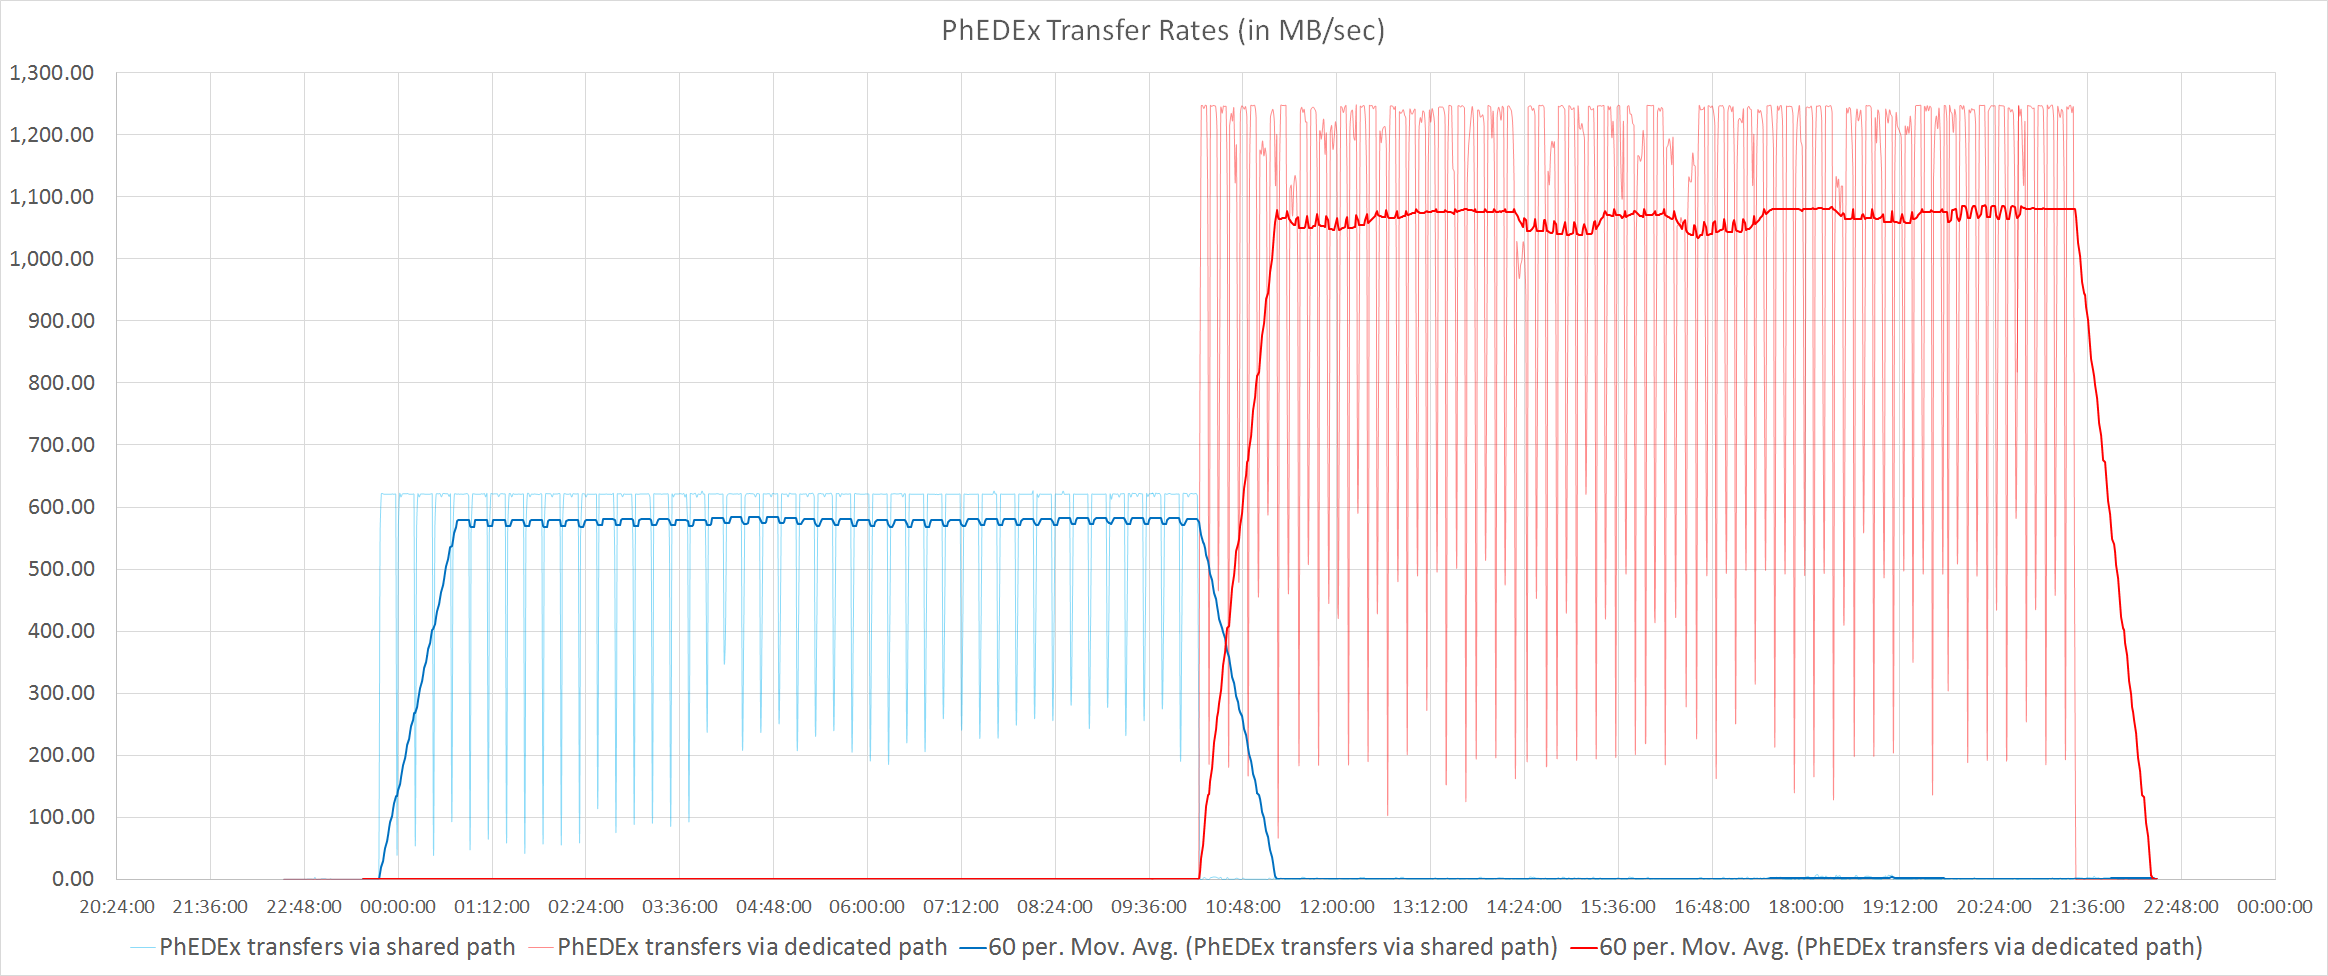
\includegraphics[width=0.95\textwidth]{figure-FileDownload_All_paths}
  \caption{View of PhEDEx transfers on a 10 Gbps link between Geneva and Amsterdam. The transfer performance on a shared path (shown in blue) is impeded by competition on the link. When a circuit becomes available on a dedicated path, PhEDEx transparently switches to using that circuit (shown in red), thereby doubling the throughput.}
  \label{fig:combined_phedex_transfers}
\end{figure} 
